The aim of the Peeragogy Handbook is to lay out effective peer-learning
techniques that you can implement ``on the ground.'' We suggest that you
look through the Handbook, try a few of these suggestions, and see how
they work for you. Then we invite you to return here, share your
experiences, ask for feedback, and work with us to improve the Handbook
and the field we affectionately call ``Peeragogy.''

In this part of the Peeragogy Handbook, teams of ``peeragogues'' have
distilled their most important and applicable research and insights from
more than a year of inquiry and discussion. Although there's been no
shortage of experimentation and formal research into collaborative,
connective, and shared learning systems in the past, we've detected a
new rumbling among education thinkers that when combined with new
platforms and technologies, peer-learning strategies as described here
could have a huge impact on the way educational institutions evolve in
the future. We've also seen for ourselves how peer learning techniques
can help anyone who's interested become an effective informal educator,
whether or not that's part of their job description.

\begin{figure}[htbp]
\centering
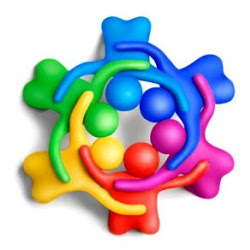
\includegraphics[width=.4\textwidth]{../pictures/peeragogy-in-action.jpg}
\end{figure}

\subsection{The interplay of individual and group}

``Personal'' supports ``peer'' - We can consciously cultivate living,
growing, responsive webs of information, support, and inspiration that
help us be more effective learners. This is a personal learning network.
We'll offer tips on how to build these networks --- and we'll also
explain how strong personal learning networks can contribute to and
evolve into even stronger peer learning networks.

``Peer'' supports ``personal'' - As we work together to develop shared
plans for our collective efforts in group projects, we usually can find
places where we have something to learn. Furthermore, if we are willing
to ask for help and offer our help to others, everybody's learning
escalates. Being mindful of effective interpersonal learning patterns is
an important part of building an effective personal learning plan.

In the following sections, you can read some more about these
strategies, or you can skip ahead to Part III to start looking at
specific techniques you can use to build your own peer learning group.

\subsection{Peer learning through the ages}

As you may have guessed, our new term, peeragogy, is a riff on the word
pedagogy --- the art, science, or profession of teaching. Pedagogy has a
somewhat problematic story of origin: it comes from the ancient Greek
tradition of having a child (paidos) be supervised (agogos) by a slave.
Greek philosophers disagreed with each other as to the best way for
individuals to gain knowledge (and even more so, wisdom). Socrates, who
insisted that he was not wise, also insisted that his interlocutors join
him in investigating truth claims, as peers. The most famous of these
interlocutors, Plato, on a more pedagogical bent, spoke of an
enlightened few, whose responsibility it was to show others the light of
knowledge (illustrated by his famous allegory of ``The Cave'').

In more recent centuries, various education theorists and reformers have
challenged the effectiveness of what had become the traditional
teacher-led model. Most famous of the early education reformers in the
United States was John Dewey, who advocated new experiential learning
techniques. In his 1916 book, Democracy and Education {[}1{]}, Dewey
wrote, ``Education is not an affair of `telling' and being told, but an
active and constructive process.'' Soviet psychologist Lev Vygotsky, who
developed the concept of the Zone of Proximal Development, was another
proponent of ``constructivist'' learning. His book, Thought and
Language, also gives evidence to support collaborative, socially
meaningful, problem-solving activities over solo exercises.

Within the last few decades, things have begun to change very rapidly.
In Connectivism: A Learning Theory for the Digital Age, George Siemens
argues that technology has changed the way we learn, explaining how it
tends to complicate or expose the limitations of the learning theories
of the past {[}3{]}. The crucial point of connectivism is that the
connections that make it possible for us to learn in the future are more
relevant than the sets of knowledge we know individually, in the
present. Furthermore, technology can to some degree and in certain
contexts, replace know-how with know-where-to-look.

If you want more details on the history, theories, and recent
experiments related to peer learning, we have a more extensive
literature review available. We've also adapted it into a Wikipedia
page, which you can edit as well as read.

\begin{figure}
\begin{center}
\href{http://commons.wikimedia.org/wiki/File:Platon\_Cave\_Sanraedam\_1604.jpg}{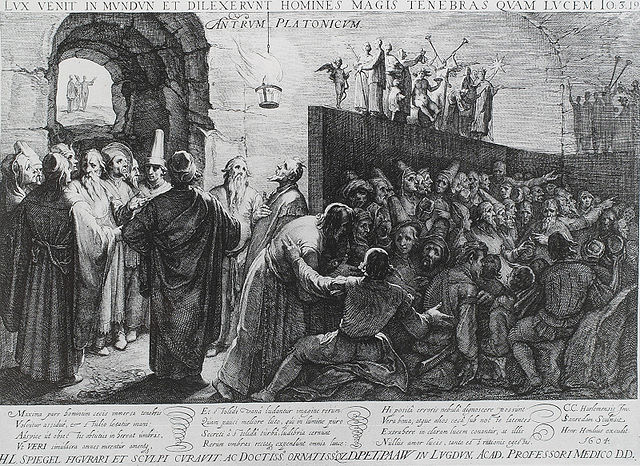
\includegraphics[width=.8\textwidth]{../pictures/plato_cave.jpg}}
\end{center}
\caption*{\href{http://commons.wikimedia.org/w/index.php?title=File:Platon\_Cave\_Sanraedam\_1604.jpg\&oldid=68567627}{Platon Cave Sanraedam (1604)}. By Jan Saenredam {[}Public domain{]}, via
Wikimedia Commons}
\end{figure}

\subsection{Which is more fun, skateboarding or chemistry?}

\begin{enumerate}
\item
  A study group for a tough class in organic chemistry convenes at at
  the library late one night, resolving to do well on the next day's
  exam. The students manage to deflect their purpose for a while by
  gossiping about college hook-ups and parties, studying for other
  classes, and sharing photos. Then, first one member, then another,
  takes the initiative and as a group, the students eventually pull
  their attention back to the task at hand. They endure the monotony of
  studying for several hours, and the next day, they own the exam.
\item
  A young skateboarder spends hours tweaking the mechanics of how to
  make a skateboard float in the air for a split second, enduring
  physical pain of repeated wipeouts. With repetition and success comes
  a deep understanding of the physics of the trick. That same student
  cannot string together more than five minutes of continuous attention
  during chemistry class and spends even less time on homework for the
  class before giving up.
\end{enumerate}
Peer-learning participants succeed when they are motivated to learn.
Skateboarding is primarily intrinsically motivated, with some extrinsic
motivation coming from the respect that kids receive from peers when
they master a trick. In most cases, the primary motivation for learning
chemistry is extrinsic, coming from parents and society's expectations
that the student excel and assure his or her future by getting into a
top college.

The student very well could be intrinsically motivated to have a glowing
report card, but not for the joy of learning chemistry, but because of
the motivation to earn a high grade as part of her overall portfolio.
Taken a different way, what is it about chemistry that's fun for a
student who does love the science? Perhaps she anticipates the respect,
power and prestige that comes from announcing a new breakthrough; or she
may feel her work is important for the greater good, or prosperity, of
humanity; or she may simply thrill to see atoms bonding to form new
compounds.

Learning situations frequently bore the learner when extrinsic
motivation is involved. Whether by parents or society, being forced to
do something, as opposed to choosing to, ends up making the individual
less likely to succeed. In some cases it's clear, but trying to figure
out what makes learning fun for a group of individual humans can be very
difficult. Often there is no clear-cut answer that can be directly
applied in the learning environment. Either way, identifying the factors
that can make learning boring or fun is a good start. Perhaps learning
certain skills or topics is intrinsically boring, no matter what, and we
have to accept that.

\begin{figure}
\begin{center}
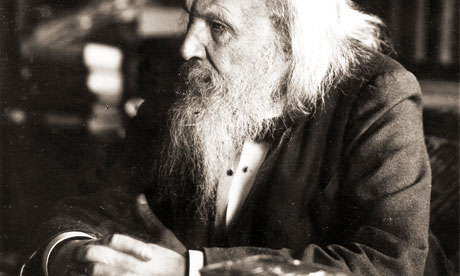
\includegraphics[width=.8\textwidth]{../pictures/mendeleev.jpg}
\end{center}
\caption*{Photo of Dmitri Mendeleev (1834-1907). Found on The Guardian's Notes \&
Theories blog. Public domain.}
\end{figure}

\subsubsection{Learning patterns}

One way to think about fun learning is that it's fun to learn - and be
aware that you're learning - new patterns. Jürgen Schmidhuber wrote: ``A
separate reinforcement learner maximizes expected fun by finding or
creating data that is better compressible in some yet unknown but
learnable way, such as jokes, songs, paintings, or scientific
observations obeying novel, unpublished laws'' {[}4{]}. So the
skateboarder enjoyed coming across new patterns (novel tricks) that he
was able to learn; tricks that challenged his current skill level.

\subsection{Learner, know thyself: a self-evaluation technique}

The learning contributed and acquired by each member of the peer
learning enterprise depends on a healthy sense of self-awareness. When
you ask yourself, ``What do I have to offer?'' and ``What do I get out
of it?'' we think you'll come up with some exciting answers. In peer
learning, whether or not you're pursuing a practical objective, you're
in charge, and this kind of learning is usually fun. Indeed, as we'll
describe below, there are deep links between play and learning. We
believe we can improve the co-learning experience by adopting a playful
mindset. Certainly some of our best learning moments in the Peeragogy
project have been peppered with humor and banter. So we found that a key
strategy for successful peer learning is to engage in a self-assessment
of your motivations and abilities. In this exercise, you take into
account factors like the learning context, timing and sequence of
learning activities, social reinforcements, and visible reward. The
peeragogical view is that learning is most effective when it contains
some form of enjoyment or satisfaction, or when it leads to a concrete
accomplishment.

When joining the Peeragogy project, Charles Jeffrey Danoff did a brief
self-evaluation about what makes him turn on to learning:

\begin{enumerate}
\item
  \textbf{Context}. I resist being groomed for some unforeseeable future
  rather than for a specific purpose.
\item
  \textbf{Timing and sequence}. I find learning fun when I'm studying
  something as a way to procrastinate on another pressing assignment.
\item
  \textbf{Social reinforcement}. Getting tips from peers on how to
  navigate a snowboard around moguls was more fun for me than my Dad
  showing me the proper way to buff the car's leather seats on chore
  day.
\item
  \textbf{Experiential awareness}. In high school, it was not fun to sit
  and compose a 30-page reading journal for Frankenstein. But owing in
  part to those types of prior experiences, I now find writing
  peasurable and it's fun to learn how to write better.
\end{enumerate}
\subsubsection{Two theories of motivation}

One of the most prominent current thinkers of (self-)motivation and
regulation is Daniel Pink {[}5{]}, who proposes a theory of motivation
based on autonomy, mastery, and purpose, or, more colorfully:

\begin{enumerate}
\item
  The urge to direct my life
\item
  The desire to get better at something that matters
\item
  The yearning to do something that serves a purpose bigger than just
  ``myself''
\end{enumerate}
There's clearly a ``learning orientation'' behind the second point: in
fact, it's not just a matter of ``fun'' --- ultimately, it's the sense
of achievement that matters.

Learning is given an even more central position in a paper by Thomas
Malone {[}6{]}, who was another thinker who asked ``What makes things
fun to learn?''. His proposed framework for motivating learning
activities is based on the three ingredients fantasy, challenge, and
curiosity --- this bears a certain analogy to Pink's framework.

We can easily see how ``participation'' relates to ``motivation'' in the
sense described here. When I get useful information from other people, I
can direct my own life better. When I have means of exploring my
fantasies and dreams by chatting then over and exploring some of the
elements in a safe way, I'm in a much better position to make something
in reality. A solid reputation that comes from being able to help others
serves as a good indicator of personal progress, and a sign that one is
able to deal with greater challenges. Relationships provide the most
basic sense of being part of something bigger than just oneself: et
cetera. (Further thoughts on the role of motivation in peer learning
appear in our chapter on Motivation.)

\subsection{Metacognition and mindfulness in peer learning}

Metacognition and mindfulness are words for awareness of how you are
thinking, attending, and participating. It can be particularly useful to
think about the roles you take on in the project, the kind of
contributions you want to make, and what you hope to get out of the
experience. These are all likely to change as time goes by.

\subsubsection{Potential roles in your peer-learning project}

\begin{enumerate}
\item
  Leader, Manager, Team Member, Worker
\item
  Content Creator, Author, Content Processor, Reviewer, Editor
\item
  Presentation Creator, Designer, Graphics, Applications
\item
  Planner, Project Manager, Coordinator, Attendee, Participant
\item
  Mediator, Moderator, Facilitator, Proponent, Advocate, Representative,
  Contributor
\end{enumerate}
\subsubsection{Potential contributions}

\begin{enumerate}
\item
  Create, Originate, Research, Aggregate
\item
  Develop, Design, Integrate, Refine, Convert
\item
  Write, Edit, Layout
\end{enumerate}
\subsubsection{Potential motivations}

\begin{enumerate}
\item
  Acquisition of training or support in a topic or field;
\item
  Building relationships with interesting people;
\item
  Finding professional opportunities through other participants;
\item
  Creating or bolstering a personal network;
\item
  More organized and rational thinking through dialog and debate;
\item
  Feedback about their own performance and understanding of the topic.
\end{enumerate}
Although this first and foremost self-evaluative examination, we find it
useful to build in a brief pause at the commencement of the project for
each peeragogue to self-define and declare what they plan to bring to
the table, what they hope to get out of the experience, how this builds
on and expands knowledge, skills, capacities, and preferences. This
process of shared reflection primes the group for cohesion and success.

\subsection{Personal Learning Networks and Peer Learning Networks}

Personal Learning Networks are the collections of people and information
resources (and relationships with them) that people cultivate in order
to form their own public or private learning networks --- living,
growing, responsive sources of information, support, and inspiration
that support self-learners.

\begin{quote}
\textbf{Howard Rheingold}: ``When I started using social media in the
classroom, I looked for and began to learn from more experienced
educators. First, I read and then tried to comment usefully on their
blog posts and tweets. When I began to understand who knew what in the
world of social media in education, I narrowed my focus to the most
knowledgeable and adventurous among them. I paid attention to the people
the savviest social media educators paid attention to. I added and
subtracted voices from my attention network, listened and followed, then
commented and opened conversations. When I found something I thought
would interest the friends and strangers I was learning from, I passed
along my own learning through my blogs and Twitter stream. I asked
questions, asked for help, and eventually started providing answers and
assistance to those who seemed to know less than I. The teachers I had
been learning from had a name for what I was doing --- ``growing a
personal learning network.'' So I started looking for and learning from
people who talked about HOW to grow a ``PLN'' as the enthusiasts called
them.''
\end{quote}

\begin{center}
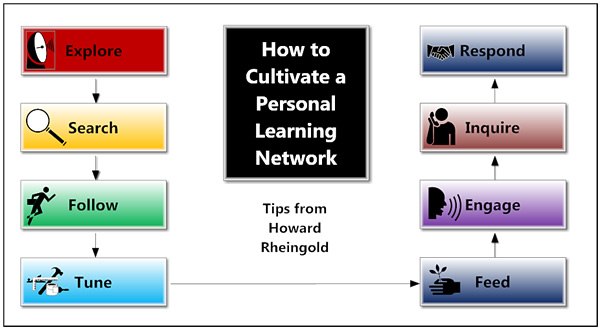
\includegraphics[width=.75\textwidth]{../pictures/network.jpg}
\end{center}

\subsubsection{Strong and weak ties}

Your PLN will have people and sites that you check on often -- your main
sources of information and learning -- your `strong ties'. Your `weak
ties' are those people and sites that you don't allow a lot of bandwidth
or time. But they may become strong later, as your network grows or your
interests expand. This is a two-way street -- it is very important that
you are sharing what you learn and discover with those in your network
and not just taking, if you want to see your network expand.

\subsubsection{Peer learning networks}

Later in the Handbook, we'll talk more about how to develop and share
``peeragogical profiles'' --- in other words how to advertise what you
want to learn, and what you'd be interested in helping teach others. A
network of people who share their profiles and experiences, and
collaboratively work, learn, teach, and communicate is a peer learning
network. You'll also find more information about building this type of a
network in our article on Peeragogy for K-12 Educators (the article is
useful even if you're not formally employed as a teacher).

\subsection{From syllabus and curriculum to personal and peer learning
plans}

Part of the effectiveness of peeragogy is that the ``syllabus'' or
``curriculum'' -- more generally, the learning plan -- is developed by
the people doing the learning. You don't faint with shock when you see
the reading list if you helped write it.

In peer learning, having a personal learning plan at the outset helps
each participant identify his or her unique learning and teaching
proclivities and capabilities, and effectively apply them in the peer
setting. In developing your personal plan, you can ask yourself the
following questions:

\begin{enumerate}
\item
  What do I most need to learn about in the time ahead?
\item
  What are the best ways I learn, what learning activities will meet my
  learning needs, what help will I need and how long will it take?
\item
  What will I put into my personal portfolio to demonstrate my learning
  progress and achievements?
\end{enumerate}
Early in the process, the peer-learning group should also convene to
develop a peer learning plan. In the Peeragogy project, we used live
meetings and forum-style platforms to discuss the group-level versions
of the questions listed above. Personal learning needs and skills were
also aired via these platforms, but the key shared outcome was an
initial project plan. Initially this took the form of an outline of
handbook chapters to write, as well as a division of labor into
different roles.

Nothing was set in stone, and both the peer group and individual
participants have continued to develop, implement, review, and adjust
their goals as the project develops. We have stayed sufficiently
connected to the original goal of producing a handbook about peer
learning that you now have one in your hands (or on your screen). We've
also added some new goals for the project as time has gone by.

Having a malleable framework enables peer learners to:

\begin{enumerate}
\item
  Identify appropriate directions and goals for future learning;
\item
  Review their strengths and areas for development;
\item
  Identify goals and plans for improvement;
\item
  Monitor their actions and review and adjust plans as needed to achieve
  their goals;
\item
  Update the goals to correspond to progress.
\end{enumerate}
This doesn't mean you have to let chaos rule, but often in the swirl of
ideas and contributions, new directIons took shape and new ideas took
hold. We expand on the notion of change in the discussion of roles and
motivations.

\subsubsection{Self-generating templates}

Documentation like mind maps, outlines, blogs or journals, and forum
posts for a peer learning project can create an ``audit trail,'' or
history, of the process. This record not only serves as a guide for new
participants, but also functions as a valuable review tool for all, and
a ready-made template for future peer-learning projects. As you mine the
documentation of a past peer-learning project or a completed phase of an
ongoing project for effective learning patterns, take the time to
validate and compare what you've achieved against the goal or mission at
the outset. Use the record to reflect and evaluate key elements of the
process for you as a facilitator and as a member of the peer learning
group. Update your plans accordingly.

\subsection{From corporate training to learning on the job}

\begin{figure}
\begin{center}
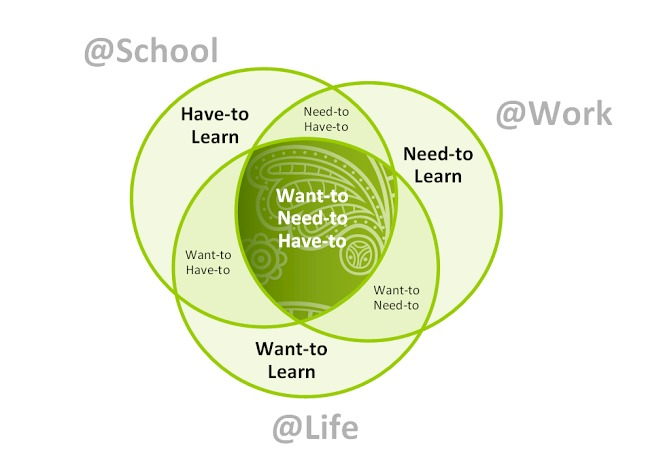
\includegraphics[width=.75\textwidth]{../pictures/learn.jpg}
\caption*{``I think because of the
tremendous changes we see in education and at work, the sets
(attitudes) are beginning to overlap more and more,'' said Joachim
Stroh of the Google+ community, Visual Metaphors.}
\end{center}
\end{figure}

Today's knowledge workers typically have instant, ubiquitous access to
the internet. The measure of their ability is an open-book exam. ``What
do you know?'' is replaced with ``What can you do?'' And if they get
bored, they can relatively easily be mentally elsewhere.

This has ramifications for the way managers manage as well as the way
teachers teach. To extract optimal performance from workers, managers
must inspire them rather than command them. Antoine de Saint-Exupéry put
it nicely: ``If you want to build a boat, do not instruct the men to saw
wood, stitch the sails, prepare the tools and organize the work, but
make them long for setting sail and travel to distant lands.''

\begin{quote}
\textbf{Jay Cross}: ``If I were an instructional designer in a moribund
training department, I'd polish up my resume and head over to marketing.
Co-learning can differentiate services, increase product usage,
strengthen customer relationships, and reduce the cost of hand-holding.
It's cheaper and more useful than advertising. But instead of just
making a copy of today's boring educational practices, build something
based on interaction and camaraderie, perhaps with some healthy
competition thrown in. Again, the emphasis should always be on learning
in order to do something!''
\end{quote}
\subsection{From peer learning to peeragogy}

The idea that we needed a new theory (which we gave the name
\emph{paragogy} {[}7{]}) arose out of the challenges we faced doing peer
learning. Our aim was to understand how groups and organizations can get
better at serving participants' interests, while participants also learn
and becoming better contributors.

Paragogy started out as a set of proposed principles that describe peer
produced peer learning -- we'll say exactly what these principles are a
bit further below. We designed them to contrast with a set guidelines
for adult educators advanced by Malcolm Knowles {[}10{]}. The paragogy
principles focused on the way in which co-learners shape their learning
context together. Peer produced peer learning is something for
``innovative educators'' everywhere, working at all scales. You don't
need to have the word teacher, trainer, or educator in your job title.
It's enough to invite someone out to lunch and ask questions, set up a
reading group with your friends, or even to tackle a new DIY project
following tips from the hardware store clerk or instructions you
downloaded from the internet.

Our secret for successful peer learning is actually hidden in plain
view: the word ``paragogy'' means ``production'' in Greek. We're
particularly interested in how the powerful blend of peer learning and
collaborative work drives open source software development, and helps
build resources like Wikipedia. But in fact it works equally well in
offline settings, from official hacker/maker spaces to garages and
treehouses. Projects like
\href{http://storycorps.org/about/}{StoryCorps} show how contemporary
media can add a powerful new layer to ancient strategies for teaching,
learning, and sharing.

The word ``peeragogy'' attempts to make these ideas immediately
understandable to everyone, including non-geeks. Peeragogy is about
peers learning together, and teaching each other. In the end, the two
words are actually synonyms. If you want to go into theory-building
mode, you can spell it ``paragogy''. If you want to be a bit more down
to earth, stick with ``peeragogy.''

\subsubsection{Different ways to analyze the learning process}

After doing some personal reflection on the roles you want to take on
and the contributions you want to make (as we discussed above), you may
also want to work together with your learning group to analyze the
learning process in more detail. There are many different phases,
stages, and dimensions that you can use to help structure and understand
the learning experience: we list some of these below.

\begin{enumerate}
\item
  I, We, Its, It (from Ken Wilber -- for an application in modeling
  educational systems, see {[}11{]})
\item
  Guidance \& Support, Communication \& Collaboration, Reflection \&
  Demonstration, Content \& Activities (from Gráinne Conole)
\item
  Forming, Norming, Storming, Performing from Bruce Tuckman.
\item
  The ``five-stage e-moderating model'' from GIlly Salmon
\item
  Assimilative, Information Processing, Communicative, Productive,
  Experiential, Adaptive (from Oliver and Conole)
\item
  Multiple intelligences (after Howard Gardner).
\item
  The associated ``mental state'' (after Csíkszentmihályi; see picture)
\item
  Considered in terms of ``Learning Power'' (Deakin-Crick, Broadfoot,
  and Claxton).
\end{enumerate}

\begin{figure}
\begin{center}
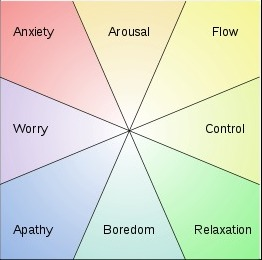
\includegraphics[width=.45\textwidth]{../pictures/challenge.jpg}
\end{center}
\caption*{\href{http://commons.wikimedia.org/wiki/File\%3AChallenge\_vs\_skill.svg}{Challenge
 vs. Skill}. By w:User:Oliverbeatson (w:File:Challenge vs skill.jpg)
{[}Public domain{]}}
\end{figure}

\subsubsection{Peer learning for one}

How can you apply the ideas of peer learning on your own? In a certain
sense, it's impossible, but somehow that never stops people from trying.
We find a striking parallel between the paragogy principles and the 5
Elements of Effective Thinking proposed by Edward Burger and Michael
Starbird in a recent book {[}12{]}. It's a nice short book and worth a
read: here, we will just quote the titles of the main chapters to
illustrate one possible parallel:

\begin{enumerate}
\item
  Changing context as a decentered center \ensuremath{\sim}
  Quintessence, Engaging Change: Transform Yourself
\item
  Meta-learning as a font of knowledge \ensuremath{\sim} Air, Creating
  Questions out of Thin Air: Be your own Socrates
\item
  Peers provide feedback that wouldn't be there otherwise
  \ensuremath{\sim} Water, Seeing the Flow of Ideas: Look Back, Look
  Forward
\item
  Learning is distributed and nonlinear \ensuremath{\sim} Earth,
  Grounding Your Thinking: Understanding Deeply
\item
  Realize the dream if you can, then wake up! \ensuremath{\sim} Fire,
  Igniting Insights through Mistakes: Fail to Succeed
\end{enumerate}
We think that ``thinking'' is often most effective when it's done with
others, and this is something that Burger and Starbird don't give much
attention. Nevertheless, even when you find yourself on your own in the
midst of that challenging DIY project, you can use the techniques of
peer learning to understand yourself as a growing, changing part of a
shared context in motion. This can contribute to an effective and
adaptive outlook on life.

We invite you to approach this book as a ``peer learner'' -- and we hope
the techniques we've introduced here will serve you well in the world at
large.

\subsection{Further reading}

\subsubsection{A word list for your inner edu-geek}

\begin{enumerate}
\item
  Constructivism
\item
  Social constructivism
\item
  Radical constructivism
\item
  Enactivism
\item
  Constructionism
\item
  Connectivism
\end{enumerate}
\subsubsection{On fun and boredom}

\begin{enumerate}
\item
  The Contribution of Judo to Education by Kano Jigoro
\item
  Pale King, unfinished novel by David Foster Wallace
\end{enumerate}
\subsubsection{On Paragogy}

\begin{enumerate}
\item
  Joe Corneli's ``Implementing Paragogy'' lesson plan, on Wikiversity
\item
  Joe Corneli and Charlie Danoff's ``Paragogy Papers'', on paragogy.net
\end{enumerate}
\subsubsection{On Learning vs Training}

\begin{enumerate}
\item
  Hart, Jane. Is it time for a BYOL (Bring Your Own Learning) strategy
  for your organization?
\end{enumerate}
\subsubsection{On PLNs}

\begin{enumerate}
\item
  Shelly Terrell: Global Netweaver, Curator, PLN Builder, blog post,
  with video
\item
  Will Richardson and Rob Mancabelli, Personal Learning Networks: Using
  the Power of Connection to Transform Education
\item
  Howard Rheingold's PLN links on Delicious
\end{enumerate}
\subsubsection{Tips from an open source perspective}

Care of User:Neophyte on the Teaching Open Source wiki.

\begin{enumerate}
\item
  The Art of Community
\item
  Open Advice
\item
  The Open Source Way
\end{enumerate}
\subsection{References}

\begin{enumerate}
\item
  Dewey, J. (2004). Democracy and education. Dover Publications.
\item
  Vygotsky, L. S. (1986). Thought and language. MIT press.
\item
  Siemens, G. (2005). Connectivism: A learning theory for the digital
  age. International Journal of Instructional Technology and Distance
  Learning, 2(1), 3-10.
\item
  Schmidhuber, J. (2010). Formal theory of creativity, fun, and
  intrinsic motivation. Autonomous Mental Development (IEEE), 2(3),
  230-247.
\item
  Pink, D. (2011), Drive: The Surprising Truth About What Motivates Us,
  Canongate Books Ltd
\item
  Malone, T.W. (1981), Toward a Theory of Intrinsically Motivating
  Instruction, Cognitive Science, 4, pp. 333-369
\item
  Corneli, J. and Danoff, C.J. (2011), Paragogy: Synergizing individual
  and organizational learning. (Published on Wikiversity.)
\item
  Knowles, M. S. (1980). The modern practice of adult education: From
  pedagogy to andragogy. Chicago: Follett.
\item
  Corneli, J., and Mikroyannidis, A. (2012). Crowdsourcing education on
  the Web: a role-based analysis of online learning communities, in
  Alexandra Okada, Teresa Conolly, and Peter Scott (eds.), Collaborative
  Learning 2.0: Open Educational Resources, IGI Global.
\item
  Burger, E. and Starbird, M. (2013). The 5 Elements of Effective
  Thinking, Princeton University Press.
\end{enumerate}
